% $Id: onchip.tex 9826 2022-02-09 20:05:05Z mskala $

%
% Manual for MSK 014 on-chip peripherals
% Copyright (C) 2022  Matthew Skala
%
% This program is free software: you can redistribute it and/or modify
% it under the terms of the GNU General Public License as published by
% the Free Software Foundation, version 3.
%
% This program is distributed in the hope that it will be useful,
% but WITHOUT ANY WARRANTY; without even the implied warranty of
% MERCHANTABILITY or FITNESS FOR A PARTICULAR PURPOSE.  See the
% GNU General Public License for more details.
%
% You should have received a copy of the GNU General Public License
% along with this program.  If not, see <http://www.gnu.org/licenses/>.
%
% Matthew Skala
% https://northcoastsynthesis.com/
% mskala@northcoastsynthesis.com
%

\chapter{On-chip peripherals}

The PIC24FJ64GB002 chip has a large assortment of built-in peripherals. 
This chapter summarizes how all the peripherals are used (if at all) in the
Gracious Host.

Microchip's documentation is a little weird.  They make many different
PIC24F chips, all with different selections of peripherals and different
details of how the peripherals can be configured.  There is the so-called
\emph{Data Sheet} (DS), which is hundreds of pages long, not really a
``sheet'' at all, for the PIC24FJ64GB002 chip.  Actually, it is for the
PIC24FJ64GB004; the -002 is a sort of poor cousin, covered by the same data
sheet.  Then there is also a \emph{Family Reference Manual} (FRM) for the
entire PIC24F family.  That describes the union of all the peripherals on
all chips in the PIC24F family.  It gives programming details for each
peripheral that are not included in the DS, so you need to read the FRM to
really write code for each peripheral; but you also need to read the DS for
specific per-chip information like how many of each kind of timer there are
and the addresses of the registers in data memory.

The chip is also old enough that it can be hard to find the correct versions
of some of the documentation on the Net.  In particular, be sure not to
confuse chapters of the PIC24F FRM with the ``dsPIC'' FRM; incautious search
engine queries are likely to return a mixture of the two.  The PIC24F FRM
does not appear to be available as a single document, and Microchip does not
make it easy to find.  You need to search for specific chapters by number. 
The DS is still readily available on their Web site.

I will go through all the chapters of the DS, describing the specific
considerations relevant to that part of the hardware in the context of the
Gracious Host.  Notes like ``(DS 3, FRM 2)'' refer to the relevant
chapter numbers in the \emph{Data Sheet} and \emph{Family Reference Manual}. 
Not every item is covered in both manuals.  In addition to these sources it
is also important to be aware of Microchip's published silicon errata; I
mention those in this summary wherever they have an impact on the Gracious
Host.

%%%%%%%%%%%%%%%%%%%%%%%%%%%%%%%%%%%%%%%%%%%%%%%%%%%%%%%%%%%%%%%%%%%%%%%%

\section{Device overview (DS 1)}

The first chapter of the DS just gives a high-level description of the
features on the chip, and describes the pinouts of the different package
variations.  Note we are using the 28-pin SPDIP.

Many pins on the microcontroller chip are general-purpose I/O (GPIO) pins
that can be reassigned to special functions with the Peripheral Pin Select
(PPS) system.  Even if left generic in the microcontroller configuration,
all 28 pins have specific purposes in the Gracious Host hardware.  So
Table~\ref{tab:mpu-pinout} gives a more specific pinout, showing the names
used by Microchip's documentation as well as the net names used in my
schematic, as well as notes on how the pins are used.  For more details of the
wiring, see the UBM with its schematics and circuit
descriptions.

\begin{table*}
{\centering
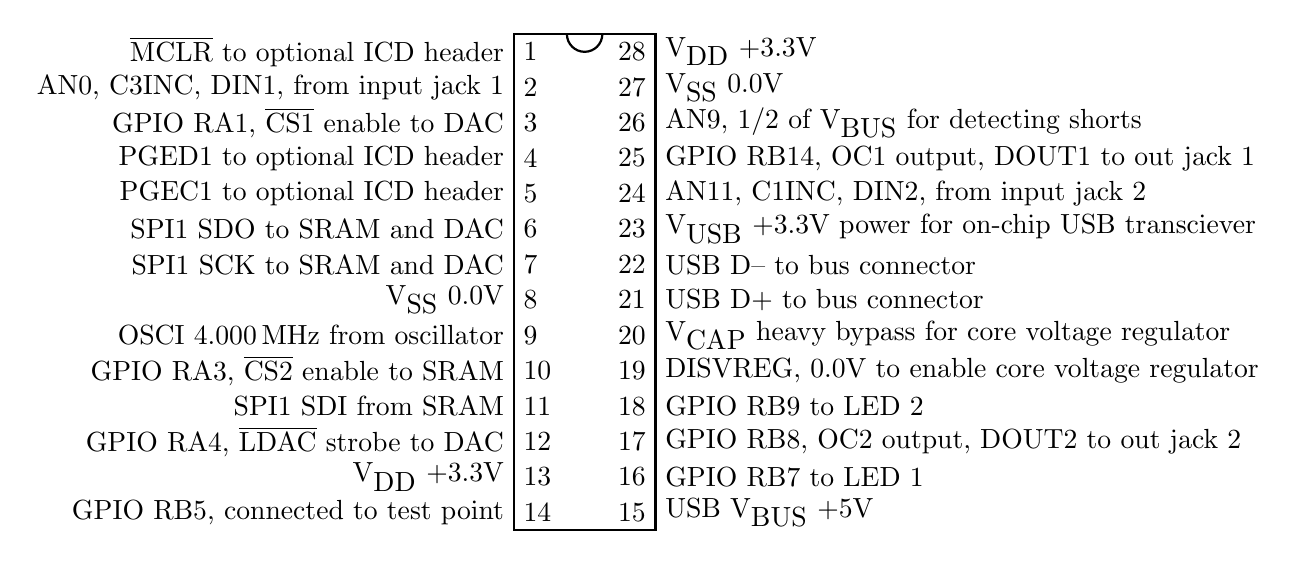
\begin{tikzpicture}[scale=4.5]
  \draw[thick] (-0.2,0.05) rectangle (0.2,-1.35);
  \draw[thick] (-0.05,0.05) arc[radius=0.05,start angle=180,end angle=360];
  \foreach \y in {1,...,14} {
    \node[anchor=west] at (-0.2,0.1-0.1*\y) {\y};
  }
  \foreach \y in {15,...,28} {
    \node[anchor=east] at (0.2,-2.8+0.1*\y) {\y};
  }
  \node[anchor=east] at (-0.2,0.0)
    {$\overline{\textrm{MCLR}}$ to optional ICD header};
  \node[anchor=east] at (-0.2,-0.1)
    {AN0, C3INC, DIN1, from input jack 1};
  \node[anchor=east] at (-0.2,-0.2)
    {GPIO RA1, $\overline{\textrm{CS1}}$ enable to DAC};
  \node[anchor=east] at (-0.2,-0.3)
    {PGED1 to optional ICD header};
  \node[anchor=east] at (-0.2,-0.4)
    {PGEC1 to optional ICD header};
  \node[anchor=east] at (-0.2,-0.5)
    {SPI1 SDO to SRAM and DAC};
  \node[anchor=east] at (-0.2,-0.6)
    {SPI1 SCK to SRAM and DAC};
  \node[anchor=east] at (-0.2,-0.7)
    {V$_\textrm{SS}$ 0.0V};
  \node[anchor=east] at (-0.2,-0.8)
    {OSCI 4.000\,MHz from oscillator};
  \node[anchor=east] at (-0.2,-0.9)
    {GPIO RA3, $\overline{\textrm{CS2}}$ enable to SRAM};
  \node[anchor=east] at (-0.2,-1.0)
    {SPI1 SDI from SRAM};
  \node[anchor=east] at (-0.2,-1.1)
    {GPIO RA4, $\overline{\textrm{LDAC}}$ strobe to DAC};
  \node[anchor=east] at (-0.2,-1.2)
    {V$_\textrm{DD}$ +3.3V};
  \node[anchor=east] at (-0.2,-1.3)
    {GPIO RB5, connected to test point};
  \node[anchor=west] at (0.2,-1.3)
    {USB V$_\textrm{BUS}$ +5V};
  \node[anchor=west] at (0.2,-1.2)
    {GPIO RB7 to LED 1};
  \node[anchor=west] at (0.2,-1.1)
    {GPIO RB8, OC2 output, DOUT2 to out jack 2};
  \node[anchor=west] at (0.2,-1.0)
    {GPIO RB9 to LED 2};
  \node[anchor=west] at (0.2,-0.9)
    {DISVREG, 0.0V to enable core voltage regulator};
  \node[anchor=west] at (0.2,-0.8)
    {V$_\textrm{CAP}$ heavy bypass for core voltage regulator};
  \node[anchor=west] at (0.2,-0.7)
    {USB D+ to bus connector};
  \node[anchor=west] at (0.2,-0.6)
    {USB D-- to bus connector};
  \node[anchor=west] at (0.2,-0.5)
    {V$_\textrm{USB}$ +3.3V power for on-chip USB transciever};
  \node[anchor=west] at (0.2,-0.4)
    {AN11, C1INC, DIN2, from input jack 2};
  \node[anchor=west] at (0.2,-0.3)
    {GPIO RB14, OC1 output, DOUT1 to out jack 1};
  \node[anchor=west] at (0.2,-0.2)
    {AN9, 1/2 of V$_\textrm{BUS}$ for detecting shorts};
  \node[anchor=west] at (0.2,-0.1)
    {V$_\textrm{SS}$ 0.0V};
  \node[anchor=west] at (0.2,-0.0)
    {V$_\textrm{DD}$ +3.3V};
\end{tikzpicture}\par}
\caption{Microcontroller pinout.}\label{tab:mpu-pinout}
\end{table*}

See Table~\ref{tab:timers} for an overview of how the Gracious Host
firmware configures many of its on-chip peripherals and which source files
do that.  The rectangular boxes show where the peripherals get their
configuration registers initialized -- sometimes more than one place if
different software modules reinitialize the peripherals -- even if the
peripherals end up being accessed elsewhere, as noted.  The oval ISR
notations show where the hard interrupt vectors point.  The ADC and output
compare hardware depends on clock frequencies that come from Timer~3 and its
prescaler, and the ISR for the comparator interrupts depends on reading time
values from Timers~4 and~5.  All the general-purpose timers are configured
to take their input from the 16.000\,MHz instruction clock.  Some other
peripherals that are less heavily linked to others, like the USB subsystem,
are not shown in this table.

\begin{table*}
{\centering
\begin{tikzpicture}[scale=1.5]
  \node at (1,0.3) {firmware.s};
  \node at (3,0.3) {ledblink.s};
  \node at (5,0.3) {midi.s};
  \node at (7,0.3) {calibration.s};
  \node at (9,0.3) {loader.s};
%
  \node[anchor=east] at (-0.1,-0.5) {T1};
  \node[anchor=east] at (-0.1,-1.5) {T2};
  \node[anchor=east] at (-0.1,-2.5) {T3};
  \node[anchor=east] at (-0.1,-3.5) {T4};
  \node[anchor=east] at (-0.1,-4.5) {T5};
  \node[anchor=east] at (-0.1,-5.5) {ADC};
  \node[anchor=east] at (-0.1,-6.5) {Comp};
  \node[anchor=east] at (-0.1,-7.5) {OC1};
  \node[anchor=east] at (-0.1,-8.5) {OC2};
  \node[anchor=east] at (-0.1,-9.5) {OC3};
  \node[anchor=east] at (-0.1,-10.5) {OC4};
  \node[anchor=east] at (-0.1,-11.5) {OC5};
%
  \draw (0,-3) rectangle (2,0);
  \draw (0,-1) -- (2,-1);
  \draw (0,-2) -- (2,-2);
  \draw (8,-1) rectangle (10,0);
  \draw (8,-3) rectangle (10,-2);
  \draw (4,-5) rectangle (8,-3);
  \draw (6,-5) -- (6,-3);
  \draw (6,-4) -- (8,-4);
  \draw (0,-12) rectangle (2,-5);
  \draw (0,-6) -- (2,-6);
  \draw (0,-7) -- (2,-7);
  \draw (0,-8) -- (2,-8);
  \draw (0,-9) -- (2,-9);
  \draw (0,-10) -- (2,-10);
  \draw (0,-11) -- (2,-11);
  \draw (4,-11) rectangle (6,-7);
  \draw (8,-8) rectangle (10,-7);
  \draw (4,-8) -- (6,-8);
  \draw (4,-9) -- (6,-9);
  \draw (4,-10) -- (6,-10);
%
  \node[anchor=west] at (0.1,-0.25) {1:256 $\div$64K};
  \node[anchor=west] at (0.1,-0.5) {0.954\,Hz};
  \node[anchor=west] at (2.1,-0.25) {sync T2};
  \node[anchor=west] at (8.1,-0.25) {1:256 $\div$64K};
  \node[anchor=west] at (8.1,-0.5) {0.954\,Hz};
  \node[anchor=west] at (0.1,-1.25) {1:256 $\div$4096};
  \node[anchor=west] at (0.1,-1.5) {15.259\,Hz};
  \node[anchor=west] at (2.1,-1.25) {LED blink};
  \node[anchor=west] at (0.1,-2.25) {1:8 $\div$412};
  \node[anchor=west] at (0.1,-2.5) {4.854\,kHz};
  \node[anchor=west] at (8.1,-2.25) {1:8 $\div$64K};
  \node[anchor=west] at (8.1,-2.5) {30.518\,Hz};
  \node[anchor=west] at (6.1,-3.25) {1:8 or 1:1 $\div$64K};
  \node[anchor=west] at (6.1,-3.5) {30.518\,Hz};
  \node[anchor=west] at (6.1,-3.75) {or 244.141\,Hz};
  \node[anchor=west] at (6.1,-4.25) {1:8 or 1:1 $\div$64K};
  \node[anchor=west] at (6.1,-4.5) {30.518\,Hz};
  \node[anchor=west] at (6.1,-4.75) {or 244.141\,Hz};
  \node[anchor=west] at (4.1,-3.25) {32-bit T4/5};
  \node[anchor=west] at (4.1,-3.5) {1:8 $\div\sim$8000};
  \node[anchor=west] at (4.1,-3.75) {~~~\,to $\sim5\times10^8$};
  \node[anchor=west] at (4.1,-4.0) {0.01--600 BPM};
  \node[anchor=west] at (4.1,-4.25) {24 PPQN clock};
  \node[anchor=west] at (0.1,-5.25) {T3 $\div$3};
  \node[anchor=west] at (0.1,-5.5) {1.618\,kHz};
  \node[anchor=west] at (0.1,-6.25) {DIN1 $\Rightarrow$};
  \node[anchor=west] at (0.1,-6.5) {DIN2 $\Rightarrow$};
  \node[anchor=west] at (6.1,-6.25) {read T4};
  \node[anchor=west] at (6.1,-6.5) {read T5};
  \node[anchor=west] at (0.1,-7.25) {$\sim$65--2093\,Hz};
  \node[anchor=west] at (0.1,-7.5) {$\Rightarrow$ DOUT1};
  \node[anchor=west] at (4.1,-7.25) {$\sim$65--2093\,Hz};
  \node[anchor=west] at (4.1,-7.5) {or 960\,$\mu$s pulse};
  \node[anchor=west] at (4.1,-7.75) {$\Rightarrow$ DOUT1};
  \node[anchor=west] at (8.1,-7.25) {$\sim$65--2093\,Hz};
  \node[anchor=west] at (8.1,-7.5) {$\Rightarrow$ DOUT1};
  \node[anchor=west] at (8.1,-7.75) {$\Rightarrow$ DOUT2};
  \node[anchor=west] at (0.1,-8.25) {$\sim$65--2093\,Hz};
  \node[anchor=west] at (0.1,-8.5) {$\Rightarrow$ DOUT2};
  \node[anchor=west] at (4.1,-8.25) {$\sim$65--2093\,Hz};
  \node[anchor=west] at (4.1,-8.5) {or 960\,$\mu$s pulse};
  \node[anchor=west] at (4.1,-8.75) {$\Rightarrow$ DOUT2};
  \node[anchor=west] at (0.1,-9.25) {($\sim$65--2093\,Hz)};
  \node[anchor=west] at (4.1,-9.25) {soft 960\,$\mu$s pulse};
  \node[anchor=west] at (4.1,-9.5) {$\Rightarrow$ CV1};
  \node[anchor=west] at (0.1,-10.25) {($\sim$65--2093\,Hz)};
  \node[anchor=west] at (4.1,-10.25) {soft 960\,$\mu$s pulse};
  \node[anchor=west] at (4.1,-10.5) {$\Rightarrow$ CV2};
  \node[anchor=west] at (0.1,-11.25) {($\sim$65--2093\,Hz)};
%
  \node[ellipse,draw,inner sep=1] at (3.55,-0.7) {\small ISR};
  \node[ellipse,draw,inner sep=1] at (3.55,-1.7) {\small ISR};
  \node[ellipse,draw,inner sep=1] at (5.65,-4.8) {\small ISR};
  \node[ellipse,draw,inner sep=1] at (1.65,-5.8) {\small ISR};
  \node[ellipse,draw,inner sep=1] at (7.55,-6.7) {\small ISR};
  \node[ellipse,draw,inner sep=1] at (5.65,-7.8) {\small ISR};
  \node[ellipse,draw,inner sep=1] at (5.65,-8.8) {\small ISR};
  \node[ellipse,draw,inner sep=1] at (5.65,-9.8) {\small ISR};
  \node[ellipse,draw,inner sep=1] at (5.65,-10.8) {\small ISR};
%
  \draw[thick,-{Stealth[scale=1.2]}]
    (2.1,-2.8) ..controls (2.4,-3.1) and (2.4,-3.5).. (2.4,-3.8)
    -- (2.4,-4.2) ..controls (2.4,-4.5) and (2.4,-4.9).. (2.1,-5.2);
  \draw[thick,-{Stealth[scale=1.2]}]
    (2.1,-2.5) ..controls (2.7,-2.9) and (3.0,-3.4).. (3.0,-4.1)
    -- (3.0,-7.0);
  \node at (3.0,-7.2) {to all OC};
  \node[anchor=east] at (2.4,-3.5) {4.854\,kHz};
  \node[anchor=west] at (2.6,-2.8) {2.000\,MHz};
\end{tikzpicture}\par}
\caption{Peripheral configuration overview.}\label{tab:timers}
\end{table*}

%%%%%%%%%%%%%%%%%%%%%%%%%%%%%%%%%%%%%%%%%%%%%%%%%%%%%%%%%%%%%%%%%%%%%%%%

\section{Microchip's guidelines for getting started (DS 2)}

This chapter discusses minimal electrical requirements for getting the chip
powered up.  The chip's main power input is nominally 3.3V, but the
microprocessor core needs a voltage of 2.55V$\pm$0.20V (at the clock speed
we are using).  It has a built-in voltage regulator to knock the 3.3V down
to the core voltage, and this voltage regulator needs to have a 10$\mu$F
ceramic (!) capacitor connected to pin~20 by as short a trace as possible to
ensure stability.  There is also a section in the errata document that is
not exactly errata, but scolds readers even more than what was already in
the data sheet regarding the need for pin 20 to be very heavily decoupled
with ultra-low inductance, and the ways in which high-$k$ ceramic capacitors
may surprise the unwary.

I have built prototypes and programming tools using a couple of film
capacitors totalling 9.4$\mu$F on pin 20, with a ZIF DIP socket and
stripboard making the connection length considerably longer than Microchip
recommands, and they seemed to work okay.  However, it is probably better to
follow the instructions as closely as possible and that is part of why I do
not use or recommend a socket for the microcontroller chip in a production
Gracious Host build.

There is further power complexity associated with the USB subsystem, which
needs to be able to handle 5.0V and can be configured to draw it from the
bus in a ``device'' configuration; but that is not terribly relevant to us,
operating as a host only.  The Gracious Host is normally intended to take
5.0V power from the Eurorack bus (also using $\pm$12V for the off-chip
analog circuitry), pass that through to the USB connector, and also use an
LDO regulator to drop it down to 3.3V for the digital chips, with the
microcontroller doing its own regulation for core voltage.

%%%%%%%%%%%%%%%%%%%%%%%%%%%%%%%%%%%%%%%%%%%%%%%%%%%%%%%%%%%%%%%%%%%%%%%%

\section{CPU (DS 3, FRM 2)}

The big thing to know about the CPU in the PIC24FJ64GB002 is that it has a
\emph{modified Harvard architecture,} which is fairly common in
microcontrollers but is different from the \emph{von~Neumann architecture}
(code and data all in one address space) more popular in general-purpose
computers.  The modified Harvard architecture has two separate address
spaces, one for code and one for data.  In the PIC24, registers and words in
data memory are 16 bits wide, as are the addresses used to point into data
memory.  Program memory is \emph{24 bits wide}; that is three bytes per
word, even though the addresses of succesive program memory words are only
two address units apart.  (So it seems like program memory addresses are
measured in units of 12 bits; but since you can't address within a program
memory word anyway, only even addresses are valid, and this is slightly less
wacky than it sounds.)

Addresses in program memory are in principle 24 bits wide for the PIC24
family.  But our chip in particular only has about 64K of program memory
(technically 22016 words, remembering they are three bytes each, so 66048
bytes), and 16 bits are enough to address all the words of program memory. 

That makes programming a little easier because program memory addresses
actually do fit in registers and it is not necessary to use ``long''
instructions that take an extra word to cover the entire theoretical address
space.  The assembly language has a lot of weird features to deal with the
tension of having 16-bit and 24-bit stuff going on at once, and there are
points where you need to explicitly do something that is like a type cast to
reinterpret numbers between the 16-bit and 24-bit worlds without generating
a fatal assembler or linker error.

You get sixteen main working registers called W0 through W15, which live at
the bottom of the data memory space.  Stuff like arithmetic usually goes
among the working registers; accessing other addresses in data memory is a
little more work.  The register W0 tends to be used as an accumulator; it is
the default destination of some operations, and has better connectivity for
things like byte-wide instructions.  The register W15 is pretty solidly
reserved for use as a stack pointer and the register W14 is the \emph{frame
pointer} for the \insn{lnk}/\insn{ulnk} stack frame instructions if you're
using those.  The Gracious Host firmware uses stack frames for exception
handling and temporary buffers.  Instructions that involve 32-bit operands
usually require an aligned pair of working registers.  Register pairs are
conventionally referred to with a colon, like W1:W0 for the 32-bit value
stored in the first two registers (little endian, so W1 is the high 16 bits
and W0 is the low 16 bits).  There are a couple of other minor reserved
purposes of specific registers but for the most part the working registers
are all alike.

The CPU can do hardware 16$\times$16$\rightarrow$32-bit multiplication in a
single instruction cycle.  There is hardware support for
32$\div$16$\rightarrow$16-bit division with remainder, but it's not as
simple as a single instruction:  it takes two
instructions and 19 instruction cycles.

The CPU has some hardware debugging support built in, including stuff like
hardware breakpoints on access to specified memory locations.  Presumably,
that is mediated by secret registers activated by the in-circuit
debugging/programming hardware and not documented or available to ordinary
code.  There is also a chunk of special RAM, accessible only through special
instructions, that buffers data about to be written to flash.  Most
peripheral devices that produce or consume data streams (like the UART and
CRC hardware) have dedicated FIFO buffers hidden behind their
input/output registers.

\emph{The PIC24 is consistently little endian everywhere, except for
a few peripherals that use other byte or bit orders required by the
standards they support.}

%%%%%%%%%%%%%%%%%%%%%%%%%%%%%%%%%%%%%%%%%%%%%%%%%%%%%%%%%%%%%%%%%%%%%%%%

\section{Memory organization (DS 4)}

This describes the memory organization \emph{native to the chip}.  More
details on how the firmware uses memory are given in other parts of this
manual.

The main program memory extends from addresses 0x000000 to 0x00ABFE.  There
are a reset vector and a couple of interrupt vector tables at the bottom of
that.  At the high end, there are a couple of words of special configuration
information.  The firmware lives between these two extremes.  The rest of
the 24-bit space is basically empty, except for a couple of special
device-ID and configuration values that can be read out of magic addresses.

The bottom of data memory, from 0x0000 to 0x07FF, is used for memory-mapped
peripherals and that kind of thing.  Interestingly, all the basic CPU
registers like the working registers and program counter and so on have
their own addresses in this space and can be accessed the same as other
data-memory locations, although sometimes incurring stuff like pipeline
stalls that slow things down a little.  Then there is 8K of general-purpose
RAM covering 0x0800 to 0x27FF.

The first 80 bytes of RAM (0x0800 to 0x084F) are used by in-circuit serial
debugging, probably for stuff like hardware breakpoints.  It is wise to
leave those reserved even in production firmware not expected to be
debugged, just in case someone wants to hook up a debugger.

Note that although I am describing the data memory using byte addresses,
most instructions can only access data memory at 16-bit aligned addresses. 
You need to use special byte-oriented instructions to touch the odd numbered
addresses, and you will get an \emph{address trap}, which leads to resetting
the CPU, if you break alignment on a word-oriented instruction.

CPU features (pre- and post-increment and decrement addressing modes on all
working registers) make it easy to support multiple stacks growing in either
direction, but the standard stack used by subroutine calls, interrupts, and
so on, is assumed to involve the register W15.  Normally, you put your
static variables at the low end of the RAM area (starting at 0x0850) and
then the stack lives after them, growing toward high addresses.  The
Microchip toolchain attempts to also support a \emph{heap} for malloc-style
allocation, but that is only really relevant when using the C compiler, and
is not really appropriate for a chip with as little RAM as this one has. 
The Gracious Host firmware includes a feature of sharing a \emph{common
data} area with local variables from different modules overlaid on top of
each other, supported by assembler macros, notwithstanding bugs and
infelicities in the Microchip toolchain that make such a thing harder to
deal with than it should be.

The USB hardware uses DMA (with a dedicated DMA controller) to access data
within the general-purpose RAM, and it needs one of its data structures to
be aligned to a 512-byte (0x200) boundary.  That complicates the RAM layout
a little.

The high half of the data memory space, that is from 0x8000 to 0xFFFF, is
used to support a feature called \emph{program space visibility} (PSV),
where you choose a 16K-word segment of program memory which will appear in
data memory space.  You only actually get to see the lower 16 bits of each
24-bit word.  There is a speed penalty for accessing these addresses.  All
in all, it's a relatively inconvenient way of reading data from program
memory, but the Gracious Host firmware does use it at one point for reading
its own hardware ID, and as part of the SRAM simulation stub (which would
not normally be assembled into firmware that would run on real hardware). 
It has the advantage that it makes program memory look just like read-only
data memory without needing special instructions.

It is also possible to read from program memory into working registers using
the \insn{tblrdl}/\insn{tblrdh} instructions, and in practice that is
usually more convenient than reading it through PSV.

Note the Gracious Host also has 128K of RAM in a separate chip, not part of
the microcontroller, that can be accessed through SPI.

%%%%%%%%%%%%%%%%%%%%%%%%%%%%%%%%%%%%%%%%%%%%%%%%%%%%%%%%%%%%%%%%%%%%%%%%

\section{Flash program memory (DS 5, FRM 4)}

The program memory is flash memory and it can be reflashed by software. 
This is a fairly dangerous thing to do and you need to go through a series
of purifying incantations described in the data sheet, under which you write
magic values to different registers on a tight schedule in order to unlock,
arm, and eventually trigger the program-memory write feature.

Most programmers will be better off to use the existing code for
loading new firmware images and doing calibration, rather than doing their
own writes to program memory.

If making direct use of the self-programming hardware features, you can't
just freely write new values overwriting old values.  After making the
sacrifices for the occasion as explained in the scripture, you have to erase
an entire aligned \emph{page} of 512 words (1.5K bytes) at a time, and then
it gets the all-ones value 0xFFFFFF in every word, and then you can rewrite
either a single word or an aligned \emph{row} of 64 words at one time.

The flash memory cannot be erased and rewritten an unlimited number of
times.  It will eventually wear out.  It's supposed to be good for ten
thousand cycles.  Use of the ``unlimited breakpoints'' feature of
Microchip's debugger can wear it out fast because this feature programs and
reprograms sections of memory every time you start and stop the program, and
I recommend avoiding that.  Beware: if you even \emph{approach} the limit on
hardware breakpoints without exceeding it, MPLAB~X~IDE will pop up a dialog
offering to enable unlimited software breakpoints without really making
clear the downside of saying ``yes.''

The last page of flash program memory (0xA800 to 0xABFE) cannot be safely
rewritten under program control because it contains the critical
configuration words; as soon as you erased it preparatory to writing new
values, you'd brick the microcontroller.  So in the Gracious Host, this page
is not used for code as such but it stores a copyright notice, an ID for the
module hardware, and a useful table of musical note frequencies (as well as
those configuration words).

The PIC24 hardware supports some so-called security features so you can make
it harder for people in the field to rewrite, or even look at, secret
things in the program memory.  Using such features would not be consistent
with the philosophy of this project.

%%%%%%%%%%%%%%%%%%%%%%%%%%%%%%%%%%%%%%%%%%%%%%%%%%%%%%%%%%%%%%%%%%%%%%%%

\section{Resets (DS 6, FRM 7)}

Chapter 6 of the data sheet goes through the different things that can cause
the microcontroller to reset, and how to read the runes after a reset to
determine which of them occurred.  Most of this stuff is primarily useful
in systems that try to do clever things with power consumption and partial
shutdowns.  The Gracious Host basically only has \emph{on} and \emph{off}
power states, so the fine details of resets between other states are not
relevant to us.

Plausible sources of resets for the Gracious Host are:
\begin{itemize}
  \item power on;
  \item catastrophic hardware failure (for instance, of the clock
    oscillator) caught by the microcontroller at a lower level
    than software can see;
  \item deliberately executing a \insn{reset} instruction, which in
    particular may happen at the
    (successful or unsuccessful) end of the firmware reflash or calibration
    sequences, from an otherwise uncaught exception throw, or during
    recovery from a detected trip of the USB polyfuse;
  \item traps on unaligned access or illegal instructions;
  \item bringing pin 1 low, which would normally only happen as part of
    in-circuit hardware debugging; and
  \item expiry of the (regular, not deep-sleep) watchdog timer.
\end{itemize}

%%%%%%%%%%%%%%%%%%%%%%%%%%%%%%%%%%%%%%%%%%%%%%%%%%%%%%%%%%%%%%%%%%%%%%%%

\section{Interrupt controller (DS 7, FRM 8)}

There are many different interrupt sources that can be turned on and off
individually and given priority levels from 0 to 7, higher numbers being
more urgent.  The CPU status includes an \emph{interrupt priority level},
normally representing the level of the interrupt currently in progress (0
during foreground code), and interrupts at or below the current CPU
interrupt level are blocked, waiting for it to decrease.  Interrupt nesting
can be disabled, but with it turned on as is default, higher-priority
interrupts can happen during the ISRs for lower-priority interrupts.  The
\insn{disi} instruction will disable all interrupts of levels 0--6, by in
effect forcing the CPU interrupt level to 7, for a number of instruction
cycles specified by a constant operand.  That can be convenient to make sure
small atomic or time-critical operations are not interrupted.

Source locations of most of the ISRs used by the Gracious Host firmware are
given in Table~\ref{tab:timers}; there is also an ISR for the USB multiplex
interrupt (which covers many different events, but they all share a vector)
in usb.s.  Priority levels used by the Gracious Host firmware are shown in
Table~\ref{tab:int-priorities}.  Priority 4 is the default for interrupts
not explicitly configured to other priorities.

\begin{table}
{\centering
\begin{tabular}{cp{1.2in}}
\multicolumn{2}{c}{MOST URGENT} \\
\hline
6 & comparators \\
\hline
5 & USB \\
\hline
4 & ADC \\
  & all output compares \\
  & Timer 5 \\
\hline
2 & Timer 1, Timer 2 \\
\hline \multicolumn{2}{c}{LEAST URGENT}
\end{tabular}\par}
\caption{Interrupt priorities in the firmware.}\label{tab:int-priorities}
\end{table}

There are two complete interrupt vector tables in low program memory, right
after the reset vector.  You can set and clear a bit in the interrupt
controller to switch between the default vector table and the ``alternate''
vector table to quickly swap between two sets of ISRs; this feature is not
used in the current Gracious Host firmware.

Microchip's linker (with this behaviour partly defined by its script) will
automatically detect the existence of symbols named like
\_\_WhateverInterrupt and \_\_AltWhateverInterrupt and use them to populate
the vector tables, using default-table entries to fill in unspecified
alternate-table entries, and using the symbol \_\_DefaultInterrupt to fill
in unspecified default-table entries.  If \_\_DefaultInterrupt is also
undefined, then the linker will create a two-instruction stub implementation
for it that Microchip's debugger disassembles as \insn{break} \insn{reset}. 
The \insn{break} instruction seems to be undocumented; it and its opcode of
0xDA0000 are not in the PIC24 \emph{Programmer's Manual}.

ISRs that do not end up resetting the CPU need to return using the
ISR-specific \insn{retfie} instruction instead of the normal \insn{return}
that would be used in foreground code.  ISRs must explicitly save and
restore registers they change that might be important to the foreground code
they are interrupting.  Note in particular that it is possible for an
interrupt to happen in the middle of a \insn{repeat} loop, and if the ISR
and foreground are both considered allowed to use \insn{repeat}, then the
ISR must save and later restore the foreground's value of the RCOUNT
register for the loop to pick up where it left off.

A general property of PIC24 interrupts is that they always happen whenever
they can, if the corresponding interrupt request bit is set in the IFSx
register.  An interrupt-causing event sets that bit, but nothing except a
reset will automatically clear it.  When the ISR starts, the CPU interrupt
priority level increases to the level that blocks the interrupt in progress,
so interrupts do not interrupt themselves, but if the ISR just returns
without explicitly clearing the interrupt request bit, then when the
\insn{retfie} instruction restores the old priority level, the interrupt
will immediately happen again.  \emph{ISRs must explicitly clear interrupt
request bits, or else they will loop forever.}

Some interrupts associated with static external states -- in particular, the
USB attach and detach interrupts -- do this same kind of thing on an
additional level, in that they will keep being requested as long as they are
enabled and the external state is in effect.  Microchip's documentation
describes this issue only vaguely, but there is code for it in their USB
driver.  Microchip calls such interrupts \emph{level triggered}.  If you
handle a USB attach interrupt, and you clear the request bit normally but
leave the attach interrupt enabled, then the request bit will immediately
set itself again and the ISR will loop.  For these kinds of interrupts, it
is important for the ISR to \emph{disable} the interrupt by clearing the
enable bit, then \emph{acknowledge} it like any ordinary interrupt by
clearing the request bit.  The disable must happen before the acknowledge
because the automatic re-request is virtually instantaneous.

%%%%%%%%%%%%%%%%%%%%%%%%%%%%%%%%%%%%%%%%%%%%%%%%%%%%%%%%%%%%%%%%%%%%%%%%

\section{Oscillator configuration (DS 8, FRM 6)}

The microcontroller has a number of different modes for its main clock,
including a built-in \emph{Fast~RC} oscillator (no external connections
needed); using an externally provided clock signal with or without internal
PLL multiplication; or using a built-in driver to drive an external crystal. 
It also has a ``secondary'' oscillator that can drive stuff like the
real-time clock when the main CPU is shut down.  And there is an elaborate
procedure for switching clock speeds on the fly, for instance as part of a
power-saving effort.

Some of these features do not work, per Microchip's published errata; some
are prohibitively fiddly and unreliable (external crystal, in particular --
I don't want to have to support DIYers likely to have trouble with that);
and use of the USB module imposes a bunch of extra requirements on the
clock, in particular a need for 0.25\%\ frequency accuracy, that cannot be
met or cannot easily be met by some of the clock options.

The Gracious Host uses what Microchip calls \emph{ECPLL mode}.  An external
oscillator module that is accurately 4.000\,MHz drives the microcontroller's
PLL, which multiplies it up to 96.000\,MHz.  I opted for 4.000\,MHz as the
lowest practical external clock frequency, to reduce EMI.  The 96.000\,MHz PLL
signal is then divided down to 48.000\,MHz, required by the USB module, and
32.000\,MHz, which is theoretically the main clock frequency of the core. 
However, almost everything in the core is actually controlled by what the
Microchip documentation calls F$_\textrm{CY}$ or F$_\textrm{OSC}/2$, both
equal to half of the main clock frequency, hence 16.000\,MHz.  The basic speed
of the CPU is one instruction per cycle of 16.000\,MHz; these cycles are
62.5\,ns each.

The clock mode is set by the configuration words in firmware.s and it is not
recommended to ever use any other mode on real Gracious Host hardware. 
However, the source file does offer a different setting to use the Fast RC
oscillator when testing this firmware on other hardware, like a generic
development board that has no external 4.000\,MHz oscillator, or in a software
simulator.  In that configuration, USB probably will not work.

%%%%%%%%%%%%%%%%%%%%%%%%%%%%%%%%%%%%%%%%%%%%%%%%%%%%%%%%%%%%%%%%%%%%%%%%

\section{Power-saving modes (DS 9, FRM 39)}

The microcontroller chip offers a bunch of special features intended to
reduce its power consumption, especially in battery-powered applications. 
Different parts of the chip can be switched on and off, clocks can be
slowed or stopped, and so on.  Most of these features are not appropriate
for the Gracious Host and some do not actually work, according to
Microchip's published errata.

The one that is used a lot in the Gracious Host firmware is \emph{idle mode}
entered by the \insn{pwrsav} \#1 instruction.  Idle mode causes the CPU to
stop executing instructions until the next interrupt, while leaving the
clock and all peripherals running.  It reduces power consumption a little
and also makes program logic simpler.  In normal operation, the ADC
interrupt at 1.618\,kHz means idle mode will never pause longer than about
618\,$\mu$s.  Coming out of idle mode resets the watchdog timer, so regular
use of idle mode makes it unnecessary to do explicit watchdog resets.

%%%%%%%%%%%%%%%%%%%%%%%%%%%%%%%%%%%%%%%%%%%%%%%%%%%%%%%%%%%%%%%%%%%%%%%%

\section{GPIO and Peripheral Pin Select (PPS) (DS 10, FRM 12)}

Some of the microcontroller's 28 pins are reserved for power; some are
reserved exclusively for specific functions, most of which are USB-related;
but most of the pins can be configured for multiple functions with general
purpose digital I/O (GPIO) as a default.  All the GPIO pins have a feature
called Change Notification (CN), which just means that they can be
configured to trigger interrupts; that is not used in the Gracious Host.

Most \emph{digital} on-chip peripherals, like serial transcievers and output
compare units but with the notable exception of the USB system, connect to
the external pins through a switching fabric and configuration mechanism
called Peripheral Pin Select (PPS).  There are 15 pins on the package
potentially available for PPS use, referred to in the DS as RP0--RP11 and
RP13--RP15 (more are available on higher-pin-count packages).

For each RPx pin, you can optionally link it to one output of an on-chip
PPS-enabled peripheral, which will override any GPIO output function the pin
would otherwise have.  Multiple pins can be linked to the same peripheral
output.  You can still read the state of a PPS-mapped output pin with GPIO
input, and you can still tri-state the pin using the GPIO tri-state control
register.  Note that many of these pins also potentially have other
functions specific to the pin that can override both GPIO and PPS.

In the other direction, for each input of an on-chip PPS-enabled digital
peripheral, you can set it to receive the signal from any one of the RPx
pins, or nothing.  You can link both a PPS input and a PPS output to the
same pin (so that one peripheral's input receives another's output) or
multiple inputs to the same pin (so that more than one peripheral input sees
the same signal, from the outside world or a PPS output).

The \emph{analog} on-chip peripherals also have some pin-selection
capability, with input multiplexers that allow them to look at different
analog-capable pins, but the analog mapping is not set up as a single named
and centrally-managed feature, and is usually not as flexible as the digital
PPS.  Note that although many microcontrollers have a more or less permanent
non-volatile pin mapping configuration feature involving so-called
\emph{fuses}, the PIC24F PPS feature is configured at run time by software,
and can be changed quickly on the fly.

The PPS mappings used by the Gracious Host are shown in
Table~\ref{tab:pps-mapping}.  The firmware sometimes changes the mappings on
the fly depending on what it's doing.  For instance, RP8 (pin 17) controls
digital output jack 2, and it is configured as GPIO when the MIDI interface
calls for sending gates through that jack, PPS mapped to OC2 when the MIDI
interface is using output compare to send trigger pulses or tones, and PPS
mapped to OC1 at the end of calibration when OC1 is being used to send the
same tone to both output jacks.  When pins are assigned to ICSP, USB, or
analog functions, those things override the GPIO and PPS functions.

\begin{table}
{\centering
\begin{tabular}{rrll}
name & no. & type & detail \\ \hline
RP0 & 4 & ICSP & debugging \\
RP1 & 5 & ICSP & debugging \\
RP2 & 6 & PPS & SPI1 data out \\
RP3 & 7 & PPS & SPI1 clock out \\
RP4 & 11 & PPS & SPI1 data in \\
RP5 & 2 & analog & input jack 1 \\
RP6 & 3 & GPIO & chip select for DAC \\
RP7 & 16 & GPIO & LED 1 \\
RP8 & 17 & GPIO/PPS & digital output jack 2 \\
RP9 & 18 & GPIO & LED 2 \\
RP10 & 21 & USB & data bus \\
RP11 & 22 & USB & data bus \\
RP12 & -- & -- & doesn't exist \\
RP13 & 24 & analog & input jack 2 \\
RP14 & 25 & GPIO/PPS & digital output jack 1 \\
RP15 & 26 & analog & USB voltage monitor
\end{tabular}\par}
\caption{Assignments of mappable pins.}\label{tab:pps-mapping}
\end{table}

It's possible for mayhem to ensue if the PPS mappings get messed up.  For
instance, although this is also a risk with ordinary GPIO, you could damage
hardware by configuring a pin as output that is also being driven in the
opposite direction by external circuitry.  The registers that change the PPS
mapping are controlled by a locking bit in the OSCCON register and the
mapping can only be successfully written when the locking bit is cleared. 
In order to change the locking bit you must first write magic values to the
register in a specified sequence.  The subroutines UNLOCK\_PPS and LOCK\_PPS
in firmware.s implement the ritual for changing the locking bit.  Normally
one would unlock the mapping, make the desired changes, and then lock it
back up again, so that if something goes wrong it's unlikely crashing code
could accidentally change the mapping in the future.

A further level of safety is available in the microcontroller by means of a
bit in one of the configuration words at the top of flash program memory
(not rewritable by software, only by ICSP) which if set creates the added
restriction that the PPS mapping registers can only be unlocked once.  After
a reset, software can unlock the mapping, set the desired mapping, then lock
it, and then future unlock sequences will not work until the next reset. 
This extra protection feature would not be appropriate for the Gracious Host
because the Gracious Host firmware needs to continue changing the mapping
repeatedly in normal operation (for instance, to support the different
PPS configurations used by different MIDI channels).

Note that pin 14, connected to the test point, is one of the few pins with
GPIO and \emph{not} PPS capability; any serial communication on that pin for
debugging or future expansion purposes will have to use bit bang. 
Having PPS capability for the test point might have been nice, but was
overridden by the need to have PPS for other pins that will be useful to
more users.

%%%%%%%%%%%%%%%%%%%%%%%%%%%%%%%%%%%%%%%%%%%%%%%%%%%%%%%%%%%%%%%%%%%%%%%%

\section{General-purpose timers (DS 11, 12; FRM 14)}

Although many peripherals have built-in timers for various purposes, the
microcontroller also has five general-purpose timers called Timer~1 through
Timer~5.  Each one is a 16-bit count-up counter with a target ``period''
value; when the counter reaches the target it resets to zero and optionally
triggers an interrupt.  There are a variety of options for exactly what gets
counted, but in the Gracious Host all the timers are normally configured to
count pulses from prescalers driven by the 16.000\,MHz instruction clock. 
The standard configuration for the general-purpose timers is shown in
Table~\ref{tab:timers} and discussed in the documentation of the different
functions they serve.

It is possible to link Timer~2 to Timer~3, or Timer~4 to Timer~5, so that
the pair will function as a single 32-bit timer instead of two 16-bit
timers.  The MIDI driver does this with Timers~4 and~5 to enable more
accurate tempo measurements.

Because the timers may be constantly updating, there is some trickery needed
to read or write the value of a 32-bit timer pair as an atomic operation
through the 16-bit microcontroller data bus.  When 32-bit mode is active,
reading or writing the \emph{low} 16-bit word of the timer value always
triggers a 16-bit transfer between the high word and a special ``hold''
register.  So to read the 32-bit value from Timer~4/5, first read TMR4 for
the low word of the 32-bit value.  That will atomically transfer the high
word into the TMR5HLD register.  Then read TMR5HLD to get the high word,
valid at the time of the TMR4 read.  Reading TMR5 directly could give
incorrect results because it might have updated between the two read
operations.  When going the opposite direction, write TMR5HLD first with the
high word, then TMR4 with the low word; the write to TMR4 will atomically
transfer the value prepared in TMR5HLD to TMR5 at the same time.  Similar
considerations apply for TMR2 and TMR3HLD when Timers~2 and~3 are configured
for 32-bit operation.  The code in midi.s demonstrates the procedure.

There are side connections from the general-purpose timers to other
peripherals.  In the Gracious Host firmware, the \emph{compare/reset events}
of Timer~3 (4.854\,kHz frequency) drive the ADC (only Timers~3 and~5 can be
selected for this), and the \emph{prescaler} of Timer~3 (1:8 ratio from the
instruction clock, thus 2.000\,MHz) drives the output compare modules.

%%%%%%%%%%%%%%%%%%%%%%%%%%%%%%%%%%%%%%%%%%%%%%%%%%%%%%%%%%%%%%%%%%%%%%%%

\section{Input capture (DS 13, FRM 34)}

The microcontroller contains five \emph{input capture} modules, which record
time stamps of edges detected on GPIO pins, with a number of options for
accumulating the time stamps in buffers, generating interrupts, and so on. 
The current version of the firmware does not use input capture at all.

We implement something similar to input capture in software using the
comparator interrupts for measuring frequencies during calibration, and in
principle we might get better timing if we could use the input capture
modules for this purpose.  But that would entail either using digital GPIO
input instead of the comparators for reading the input jacks (which makes
them less tolerant of badly chosen voltages), or else running each
comparator output to an unused PPS remappable pin (of which there are none)
to allow the input capture module to time comparator events.  Some kind of
workaround might be possible by temporarily repurposing PPS pins normally
used for something else, such as the SPI bus output pins.  Those should be
harmless to drive to random digital levels when the enable lines are not
asserted; but exploring that possibility is a project for some future
version of the firmware.

%%%%%%%%%%%%%%%%%%%%%%%%%%%%%%%%%%%%%%%%%%%%%%%%%%%%%%%%%%%%%%%%%%%%%%%%

\section{Output compare (DS 14, FRM 35)}

The \emph{output compare} modules are basically the inverse of input
capture:  they generate digital signals, which can be mapped to different
pins of the microcontroller, at pre-scheduled times determined by timing
counters reaching specific values.  There are five such modules, with a
variety of input and output options.

In the Gracious Host firmware, all five output compare modules (although
only four are ever really used) are configured to take their clock input
from \emph{the prescaler of} general-purpose Timer~3, which is configured
for 1:8 prescaling of the instruction clock.  Therefore the output compare
counters all count at 2.000\,MHz.  The first two (OC1 and OC2) are, when in
use, PPS mapped to the DOUT1 and DOUT2 pins to make their outputs appear on
the trigger/gate output jacks.  They are configured either to a PWM mode,
actually used here as a frequency generator, to generate musical notes; or
else to generate 960\,$\mu$s pulses for use as triggers.

The next two modules (OC3 and OC4) are, when used at all, configured to
generate 960\,$\mu$s pulses but not actually mapped to output pins. 
Instead, there is a soft connection (mediated by code in midi.s including
two ISRs) allowing them to send pulses to the DACs: if the MIDI subsystem
wants to send a trigger pulse to an analog output jack, it configures the
output compare module to send a pulse and interrupt at the end of the pulse,
then sends a high-voltage command to the DAC over SPI.  In the ISR that runs
at the end of the pulse, the MIDI subsystem sends a low-voltage command to
the DAC to end the pulse.  This way the analog and digital output jacks get
as near as possible the same accurate timing for their pulses, with minimal
effort by the CPU, even though the microcontroller is connected to the
analog output jacks only through the DAC.

The last page of flash program memory contains a table starting at 0x00A808
(NOTE\_TBL) that gives period values for configuring the output compare
modules to play different MIDI notes in PWM mode.  With 16-bit counters
clocked at 2.000\,MHz, the lowest achievable MIDI note pitch is note 23, B0
at 30.868\,Hz, although the table contains dummy data for notes 0 to 22 to
make indexing easier.

There are some significant published errata for the output compare modules. 
One says that the feature of linking pairs of 16-bit output compare
modules to create 32-bit output compare modules basically does not work, or
works only with severe limitations.  The current Gracious Host firmware does
not attempt that.

The FRM, when describing the output compare ``dual compare single pulse
mode,'' which we use for generating trigger pulses, says in a comment of the
C-language example code that ``It is a good practice to clear off the
control bits initially.''  That understates the situation.  In fact, it is
not just ``good practice,'' but \emph{absolutely necessary}, to clear the
control bits before requesting a pulse, and this is necessary before every
pulse, not only when initially configuring the module.  The pulse is
triggered by the \emph{actual change} of the low three bits of OCxCON1 from
0x0 to 0x4, not just (as one might reasonably interpret the documentation)
by doing a write operation of the value 0x4.

To make matters worse, there is a silicon erratum saying that the module may
generate a requested interrupt a short time before it becomes able to
process the clearing of the control bits, and I have confirmed this with
hardware testing.  What can happen is that at the end of the output pulse it
generates an interrupt, the ISR immediately attempts to clear the control
bits, but the bits don't change because the module was still thinking, and a
subsequent attempt to request another pulse will fail.

The workaround implemented in midi.s is for each output compare ISR to
execute a short do-nothing loop to pause 1\,$\mu$s (two prescaler cycles at
1:8, which should be enough) before and after clearing the mode bits.  When
the foreground receives control after the ISR returns, the module will be
ready to correctly accept a request for a new pulse.

%%%%%%%%%%%%%%%%%%%%%%%%%%%%%%%%%%%%%%%%%%%%%%%%%%%%%%%%%%%%%%%%%%%%%%%%

\section{Serial Peripheral Interface (SPI) (DS 15, FRM 23)}

SPI is a serial bus commonly used for microcontrollers to
talk to off-chip peripherals.  The microcontroller in the Gracious Host has
two built-in SPI modules, but because of the limited availability of
external pins, the Gracious Host only uses one of them, shared between the
SRAM and DAC chips.  SPI unit 1 is PPS mapped to pins 6, 7, and 11 of the
microcontroller; pins 3, 10, and 12 are also used in GPIO mode to support
SPI communication as chip selects (so that the SRAM and DAC will each ignore
transactions directed at the other) and a strobe for synchronizing the DAC
value changes.  See the chapter on off-chip peripherals for description of
the SRAM and DAC.

The SPI bus is in principle bidirectional, but in our application only the
SRAM is hooked up to communicate in both directions.  The DAC is effectively
write-only.  The SPI bus \emph{master}, which in the Gracious Host is
always the microcontroller, controls timing by transmitting a clock signal,
and the SPI peripheral transmits and receives one bit on each clock pulse --
whether those bits contain useful information or not.  Writes to the SRAM or
DAC must be matched by corresponding reads, else the read buffer will
overflow, and reads from the SRAM must be triggered by writing the same
number of bits.

It is a published silicon erratum that when the microcontroller wakes up
from ``sleep mode,'' the SPI module sometimes transmits and receives a
couple of bogus bytes or words.  That is not relevant to the Gracious Host,
which does not use sleep mode.

Another erratum says that the SPITBF bit, which reports whether the transmit
buffer is full, sometimes incorrectly indicates space available a little too
early when the prescaler is set to a slower ratio than 1:4.  The Gracious
Host uses a prescale ratio of 1:2 (from the 16\,MHz clock, hence 8\,Mbps
data rate), which should make this erratum irrelevant, but during testing I
nonetheless had problems with what may have been missed bytes when I was
trying to fill the buffer all the way using SPITBF.  Although I don't know
that that was really a silicon problem (it could instead have been some
unknown mistaken logic in my code), I rewrote the code in question to never
use SPITBF and never fill the buffer completely, and it now works.  Filling
the buffer completely does not seem to be necessary and is probably better
avoided.

%%%%%%%%%%%%%%%%%%%%%%%%%%%%%%%%%%%%%%%%%%%%%%%%%%%%%%%%%%%%%%%%%%%%%%%%

\section{Inter-Integrated Circuit (I$^2$C) (DS 16, FRM 24)}

The I$^2$C bus is another serial bus for communicating with off-chip
peripherals, like SPI but not the same as SPI.  There are no I$^2$C off-chip
peripherals in the Gracious Host and this bus probably cannot be used in any
meaningful way.

%%%%%%%%%%%%%%%%%%%%%%%%%%%%%%%%%%%%%%%%%%%%%%%%%%%%%%%%%%%%%%%%%%%%%%%%

\section{Universal Asynchronous Receiver Transmitter (UART) (DS 17, FRM 21)}

UART is yet another serial interface, typically run at relatively low speed
and used for communicating with human users via terminal-like interfaces. 
Its basic design can be traced back to early Teletype communication
standards.  With a voltage level translation, it can be connected to RS-232. 
There are two UART units on the chip.  The standard firmware does not use
them at all, but in principle, a firmware that wanted to expose a terminal
interface might be able to activate a UART and PPS-map it to the front-panel
jacks.

Microchip has documented an erratum that the UART modules cannot send two
consecutive \emph{break} signals.  That is unlikely to be a problem.

%%%%%%%%%%%%%%%%%%%%%%%%%%%%%%%%%%%%%%%%%%%%%%%%%%%%%%%%%%%%%%%%%%%%%%%%

\section{Universal Serial Bus (USB) (DS 18, FRM 27)}

One of the major features of this microcontroller chip is its USB support. 
It is designed to support USB 2.0 device or host operation, including
switching between the two roles according to ``USB On The Go.'' The hardware
supports \emph{low speed} (1.5\,Mbps) and \emph{full speed} (12\,Mbps); not
USB 2.0 \emph{high speed} (480\,Mbps) nor USB 3.0 \emph{SuperSpeed}
(5.0\,Gbps).

The PIC24F USB module uses a dedicated DMA controller to read and write data
in general-purpose RAM.  It expects a data structure called the Buffer
Descriptor Table (BDT) to exist at an address that is configurable, but must
be 512-byte aligned.  The BDT contains pointers to buffers for the actual
data to be transferred, which can be anywhere in RAM (including unaligned
byte addresses).  Semaphore bits in the BDT record whether the CPU or the
USB module own each buffer; in a typical transaction, the CPU sets up the
buffer, flips the bit to transfer ownership to the USB module, writes a
register to actually start the transaction, and then waits for the buffer to
return to CPU-owned status.

The USB module also leans very heavily on the use of interrupts.  It
basically has its own interrupt controller, with many different interrupt
sources that can be turned on and off and are all multiplexed onto a single
PIC24F interrupt request and interrupt vector.  Much of the logic of the USB
driver ends up being written into the ISR for the USB multiplex interrupt;
foreground code basically just sets up data structures and then waits for
the ISR to set flags indicating the transfer is complete, in much the same
pattern as the lower-level relationship between the CPU and USB module.  See
the notes in the ``interrupt controller'' section of this chapter regarding
\emph{level triggered} interrupts.

Microchip provides a C-language USB driver for the PIC24F, and that driver
is the only way they recommend using this hardware.  The hardware is not
really documented in enough detail to allow a programmer to write a driver
for it.  Nonetheless, I've done it, and the resulting code is included in
the Gracious Host firmware and discussed elsewhere in this manual.

Implementing a full USB protocol stack on a microcontroller this size is a
tall order because of the number of cases that need to be handled.  The
Gracious Host's implementation is stripped down to the bare essentials and
may not be as error-tolerant, nor as broadly compatible with a wide range of
devices, as users might expect from the USB implementation on a PC.  One
important limitation is that the Gracious Host's USB driver, in its current
version, does not support USB hubs at all.  Another is that it does not
support isochronous transfers (typically used by sampled audio interfaces).

The PIC24F USB hardware supports something called \emph{ping-pong buffers},
where each endpoint and direction has (potentially, depending on
configuration) two buffers.  The CPU is supposed to be able to work on one
buffer while the USB unit is doing DMA on the other, to maximize throughput. 
As far as I can tell, although Microchip's driver can be configured to set
the register bit that enables this hardware feature, it cannot \emph{really
take advantage of} it -- even in ping-pong mode the Microchip driver waits
for each transfer to fully complete before setting up the next.  My own
driver does not (in the current version) even attempt to enable ping-pong
mode.  In the intended application, there is no need for maximized
throughput.

One thing that can go wrong on a USB interface is that someone can short out
the power connection -- or just plug in a device that tries to charge a
battery, at high current, without first following the protocol to request
extra power from the host.  To guard against such situations, the Gracious
Host hardware (as is required by the USB specification, though I do not
accept an obligation to follow the specification on every point) includes a
polyfuse on the USB power line that should trip and cut off the current if
the external USB device draws too much.  See the description of the ADC,
below, regarding the firmware's handling of a polyfuse trip.

Communicating with low-speed USB devices, such as (typing) keyboards and
mice, requires sending signals called \emph{keep-alives} at 1\,ms intervals. 
The DS and FRM do not mention keep-alives, and even the USB 2.0 standard
barely mentions them.  I have determined by experiment, with a lot of
oscilloscope measurements, that when the PIC24F USB module is in low-speed
mode, the register bits that tell it to send SOFs (required every
millisecond in full-speed mode) will actually make it send keep-alives
instead.  That is probably the most convenient way for it to work.  One
small gotcha is that it is capable of sending keep-alives into an empty bus
after the device has disconnected.  The firmware has to turn keep-alives (or
SOFs) off in this state.

Detection of the speed of a connected USB device (low-speed or full-speed)
is quite finicky and may give incorrect answers if done at the wrong point
in the attach/enumeration sequence, possibly because speed detection depends
on recognizing the idle state of the bus, which is opposite for the two
speeds.  Once there is data being sent on the bus the CPU can no longer
depend on its being idle at any given moment.  Similarly, and probably for
the same reason, reading the bus to detect whether the device is attached or
not seems to be very unreliable; devices often temporarily seem unattached
based on bus state, and a driver that is too eager to detect a detach will
often do so spuriously.  The only reliable way to detect device attach and
detach seems to be the attach and detach interrupts, but those are only
reliable when very carefully handled because of their \emph{level triggered}
nature, as well as some corner cases that can arise when a driver tries to
maintain a soft attach/detach state (as is necessary, because the driver
can't just read the bus, because reading the bus doesn't work).

The USB module can potentially generate two different timer tick interrupts
at 1\,ms intervals: the ``USB On The Go 1\,ms interrupt'' and the ``Start Of
Frame (SOF) interrupt.'' These two interrupts are not synchronized, are not
both accurately at 1\,ms intervals, and tend to drift back and forth
relative to each other.  I think the SOF interrupt is more accurate for
timing, but it only happens when a device is attached and SOFs or
keep-alives are turned on, whereas the USB OTG 1\,ms interrupt can be
enabled any time the USB module is powered up.

The Gracious Host USB driver would like to have 1\,ms interrupts for timing
delays, even during device attach when SOFs are not available.  In an
earlier stage of development I just used the OTG 1\,ms interrupt all the
time because it was available in all attach/detach states, but I later found
that I needed to handle the SOF interrupt also for doing other things, and I
had bugs that were triggered when the two interrupts drifted into a certain
phase relationship.  As a temporary workaround I implemented a more
complicated scheme that would switch between using the SOF interrupt for
timing when it was available, and the OTG 1\,ms interrupt for timing
otherwise.  I eventually fixed the interrupt-phase bugs, so having both
interrupts turned on at once was no longer a problem, but I kept the
interrupt-switching logic because of the better timing accuracy of the SOF
interrupt, and to reduce the number of calls to the ISR.  Because of the
important role of waiting in CPU idle mode for USB interrupts, very much of
the timing of events throughout the Gracious Host firmware ends up being
on 1\,ms boundaries driven by the SOF interrupt.

It is a published erratum that the USB module in host mode cannot
communicate with a low-speed device through a hub, and the only workaround
offered is to connect the low-speed device directly to the microcontroller
without a hub.  The current Gracious Host firmware does not allow the use of
hubs anyway, as a matter of the feature being unimplemented in the driver;
but this issue represents a pretty significant limitation on what might be
implemented in the future.  Even with a driver that could support hubs, we
couldn't connect anything else with one low-speed device connected, so
readily imaginable scenarios like ``keyboard and mouse'' are out of reach. 
Multiple USB MIDI devices attached to a hub might still be a possibility,
because they are normally full-speed rather than low-speed devices.

Another published erratum says that because of incorrect CRC5 calculation,
external transceivers cannot be used -- and again, there is no workaround
except ``don't do that.''  (The Gracious Host doesn't, anyway.)  There are a
couple of other USB errata related to device mode and details of detecting
certain states of the interface, but they don't look relevant to the
Gracious Host or like they would limit achievable functionality.

Although this point is not mentioned in the errata, I have observed the
PIC24F USB module to sometimes overrun its buffers.  When it should be
reading a packet of a given size from the bus, it may DMA-write correct data
of the specified length to RAM, and report that the correct amount was
transferred, but actually also write some garbage after the correct data. 
Although I was not able to fully characterize the circumstances that cause
the problem, it seemed like it might be related to low-speed transfers,
unaligned buffer starts, or unaligned buffer ends.  The largest overrun I
saw was three bytes.  Trashing memory after the end of the buffer is
especially damaging when the buffer is allocated in a stack frame, because
the next thing after the buffer is likely to be an important return address. 
The Gracious Host firmware works around this issue by allocating a little
extra space for each buffer, either seven or eight bytes as needed to ensure
alignment.  That can accommodate more than twice the maximum observed
overrun, and in testing it seems to be enough.

%%%%%%%%%%%%%%%%%%%%%%%%%%%%%%%%%%%%%%%%%%%%%%%%%%%%%%%%%%%%%%%%%%%%%%%%

\section{Parallel Master Port (PMP) (DS 19, FRM 13)}

The Parallel Master Port seems to be meant to expose an address and data bus
to the outside world for accessing old-fashioned memory-mapped
microprocessor peripherals.  This module cannot be used on the Gracious
Host.  Some of its pins don't even exist on the 28-pin version of the
microcontroller package, and others are permanently wired to other functions
on the circuit board.

%%%%%%%%%%%%%%%%%%%%%%%%%%%%%%%%%%%%%%%%%%%%%%%%%%%%%%%%%%%%%%%%%%%%%%%%

\section{Real-Time Clock and Calendar (RTCC) (DS 20, FRM 29)}

The RTCC is meant to handle human-style timekeeping (days, hours, etc.),
especially with the ability to keep running while the microcontroller is in
low-power modes.  Since we don't use the low-power modes, have no provision
for keeping the microcontroller powered up even a little bit when the
Gracious Host is not fully powered up, and we cannot spare pins for the
external low-frequency crystal that the RTCC normally prefers to use, the
RTCC module certainly can't work at its best and may not be usable at all. 
The standard firmware does not attempt to use it.

%%%%%%%%%%%%%%%%%%%%%%%%%%%%%%%%%%%%%%%%%%%%%%%%%%%%%%%%%%%%%%%%%%%%%%%%

\section{Cyclic Redundancy Check generator (CRC32) (DS 21, FRM 41)}

The CRC32 module is meant to generate and check almost all forms of cyclic
redundancy checks of up to 32 bits, more efficiently than would be possible
in plain software.  Actually using this module is tricky; not everything
said about it in Microchip's documentation appears to be true, and even if
true the documentation is incomplete; and the consensus among PIC24
programmers seems to be that it's not worth the effort and you're better off
just writing a software implementation and accepting the lower performance. 

Nonetheless, I got the hardware CRC working and the Gracious Host
firmware uses it for checking integrity of firmware images and as part of
the random number generator.  Both these use a configuation intended to
match the CCITT CRC32 algorithm as used by Ethernet, Gzip, ZModem, and many
other systems.  It is probably best not to touch the CRC hardware directly,
but access it through the APIs provided by loader.s and utils.s and
documented elsewhere in this manual.

The CRC32 module is separate from the dedicated CRC hardware that is built
into the USB module and not directly visible to the CPU.

%%%%%%%%%%%%%%%%%%%%%%%%%%%%%%%%%%%%%%%%%%%%%%%%%%%%%%%%%%%%%%%%%%%%%%%%

\section{Analog to digital converters (ADC) (DS 22, FRM 17)}

The microcontroller contains a single 10-bit ADC with a complicated
multiplexer arrangement that allows it to automatically scan through a list
of inputs on a defined schedule, accumulate measurements into a buffer, and
then interrupt the CPU when it has filled the buffer.  In the Gracious Host,
this is more or less permanently configured to cycle through reading
voltages on pin~2 (AN0, DIN1, scaled and inverted voltage from input jack
1), pin~26 (AN9, scaled voltage from the USB power connection downstream of
the polyfuse), and pin~24 (AN11, DIN2, scaled and inverted voltage from
input jack 2).

Timer~3 generates a 4.854\,kHz frequency to drive the sampling; each of the
three inputs is sampled at one third of that rate, hence 1.618\,kHz, and
interrupts are generated at 1.618\,kHz to be handled by an ISR in firmware.s. 
The ISR updates the global variables INPUT\_ADC1, INPUT\_ADC2, and
USB\_VBUS\_ADC with the values from the hardware.  This update frequency was
chosen to be in a Golden Ratio relationship to the 1.000\,kHz USB start of
frame interrupt, reducing the possibility for creating a rational
beat-frequency interaction between the two.

For INPUT\_ADC1 and INPUT\_ADC2, the scaling is nominally 206 corresponding
to 5.0V on the input jack and 989 corresponding to 0.0V on the input jack
(note the inversion).  But the raw ADC values are affected by component
value tolerance and ADC nonlinearity, and the ADC1\_TO\_NOTENUM and
ADC2\_TO\_NOTENUM subroutines in calibration.s can apply calibration data to
these numbers to get more accurate measurements.  The external circuitry
should protect the microcontroller from damage for any voltage
within $\pm$12V at the input jacks, but it is only intended to guarantee
useful ADC measurements over 0.0V to 5.0V.

For USB\_VBUS\_ADC, the scaling is 0 corresponding to 0.0V on the
microcontroller pin and bus, up to 1023 corresponding to 3.3V on the
microcontroller pin, 6.6V on the bus.  The theoretically ideal reading is
775 corresponding to a bus voltage of 5.0V.  The ISR will detect a short if
the reading is less than or equal to 558 (corresponding to a bus voltage of
3.6V and normally indicating that the polyfuse has tripped) for at least
100ms; in that case it stops everything, waits until the bus voltage stays
at or above 4.0V (raw ADC reading 620) for at least 1000ms, and then resets
the microcontroller.

In a real-life bus power short situation, the extra
load on the power supply may screw things up badly enough (in particular, by
driving the upstream 5.0V regulator into protective shutdown) that the
microcontroller is not able to complete this recovery sequence under program
control; but it will eventually reset anyway according to the normal
power-up sequence after the power voltages get back under control.  If the
5.0V supply ends up permanently damaged, too bad, but the polyfuse will
probably protect the 5.0V supply and the 3.3V regulator will probably
protect the microcontroller.

It is probably better to just read the variables written by the existing
ISR, rather than attempting to access the ADC hardware directly.

%%%%%%%%%%%%%%%%%%%%%%%%%%%%%%%%%%%%%%%%%%%%%%%%%%%%%%%%%%%%%%%%%%%%%%%%

\section{Analog comparators (DS 23, FRM 46)}

The microcontroller includes three analog comparators which continuously
check outside pins against reference voltages.  These operate in parallel
with the ADC inputs.  For taking basically digital inputs (gates and
triggers) from the input jacks, it is preferable to use the comparators
rather than the ADC measurements because the comparators are faster and can
generate interrupts; and it is preferable to use the comparators rather than
treating the pins as GPIO pins to be read digitally, because the comparators
provide better-defined threshold behaviour.

Microcontroller pin~2 (AN0, DIN1) is driven by input jack~1 and connected to
comparator unit~3.  Microcontroller pin~24 (AN11, DIN2) is driven by input
jack~2 and connected to comparator unit~1.  Comparator unit~2 is not useful
in the Gracious Host; it could only be assigned to pins that are permanently
wired for ICSP and SPI purposes.  Note that the buffers from the input jacks
to the microcontroller pins are inverting, but the comparators are also
configured with inverted input assignments, so the comparator outputs end up
in positive sense relative to the input jacks.

Current values of the comparator outputs are available in bit COUT of the
CM3CON and CM1CON registers for DIN1 and DIN2 respectively.  The
comparators are set up in inverting mode, undoing the inversion of the input
buffers, so these bits are set for high input at the jacks and clear for low
input at the jacks.  The comparator references (see below) are configured
for a threshold voltage equivalent to 1.62V nominal at the input jacks.

The ISR for the comparators is in calibration.s.  It runs on falling edges
at the microcontroller pins, rising edges at the input jacks.  It records
timestamps from Timers~4 and~5 to provide something like input capture
implemented in software for frequency measurement during calibration, and it
sets soft interrupt flags used by some MIDI modes.

Microchip has published a silicon erratum saying that when the internal
bandgap reference (see below) is enabled for the comparator reference
module, the comparator may not generate interrupts properly.  They suggest a
distressingly expensive workaround of routing the comparator output to an
external pin and then using the general interrupt-on-pin capability to
detect when it changes.  That problem is not directly relevant to our
configuration, because we don't need to use the bandgap reference; but we
have had a different problem that may be related, of the comparator
generating interrupts on \emph{both} edges of an input pulse when only
interrupts on the \emph{falling} edge (at the pin; rising at the input jack)
were requested.  The ISR in calibration.s works around spurious interrupts
by checking the comparator output on every interrupt to confirm it was
really a falling edge.

%%%%%%%%%%%%%%%%%%%%%%%%%%%%%%%%%%%%%%%%%%%%%%%%%%%%%%%%%%%%%%%%%%%%%%%%

\section{Comparator voltage reference (DS 24, FRM 20)}

There are multiple options for generating voltage references for the
comparators, including using external pins, a built-in bandgap reference, or
the microcontroller's power supply, as well as scaled versions of these.  As
discussed above, an erratum causes the built-in bandgap reference to
conflict with interrupt generation.  The Gracious Host firmware configures
this module to use a scaled version of the power supply, equivalent to 1.62V
nominal as seen at the input jacks, and it would rarely be a good idea to
change this configuration.

%%%%%%%%%%%%%%%%%%%%%%%%%%%%%%%%%%%%%%%%%%%%%%%%%%%%%%%%%%%%%%%%%%%%%%%%

\section{Charge Time Measurement Unit (CTMU) (DS 25, FRM 11)}

I don't know much about the Charge Time Measurement Unit, but it seems to be
a kind of specialized ADC that measures capacitance by feeding a known
current into an unknown-sized capacitor and measuring how long it takes for
the voltage to change a known amount.  This is meant to be used for
implementing touch sensors.  It is unlikely to be usable in the Gracious
Host because the pins it can work with are all needed by other things.

%%%%%%%%%%%%%%%%%%%%%%%%%%%%%%%%%%%%%%%%%%%%%%%%%%%%%%%%%%%%%%%%%%%%%%%%

\section{``Special features,'' notably in-circuit programming (DS 26; FRM 9,
29, 32, 33)}

This chapter of the \emph{Data Sheet} describes configuration and
programming features of the chip, as well as re-iterating some of the
information about the onboard voltage regulator that cuts the 3.3V power
supply down to the core's internal voltage.  The chip has some features,
described in DS~26, for ``protecting'' firmware code from being read by
reverse engineers.  Such an effort is not consistent with the goals of this
project.

Low-level configurable hardware features, such as the clock source, are set
by ``configuration bits'' at the very top of the programmable area of flash
memory.  These are often called configuration ``fuses'' on microcontrollers
in general because of their historical implementation using fusible-link
PROM (one time programmable) but on the PIC24 in particular, they are
actually just bits in reprogrammable flash memory, copied into volatile
registers at power-up.

The configuration bits for the Gracious Host firmware are set in firmware.s,
and the recommended configuration for a standard production module is as
follows.  The config.inc file offers a few options that can change these for
debugging or development purposes.

Configuration word 1:
\begin{itemize}
  \item JTAG disabled (JTAG conflicts with external hardware connnections)
  \item code ``protection'' disabled
  \item writes to program memory allowed
  \item reset into operational mode (this may be implicitly changed by the
    Microchip in-circuit debugging tools when used in debug mode)
  \item in-circuit debugging uses PGEx1 pins (these are the ones connected
    for this pupose on the board, and a published erratum says the PGEx3
    pins conflict with the operation of the ADC)
  \item watchdog timer (WDT) enabled
  \item WDT prescaler 1:128, postscaler 1:256, which gives 1.024\,s nominal
    watchdog timeout
\end{itemize}

Configuration word 2:
\begin{itemize}
  \item ``two-speed startup'' disabled (published erratum says it does not
  work)
  \item PLL prescaler 1:1 (for 4.000\,MHz external clock input)
  \item PLL starts automatically
  \item use PLL for clock
  \item clock switching disabled
  \item don't use external clock output
  \item allow repeated reconfiguration of PPS mapping
  \item default pins for I$^2$C (not used anyway)
  \item use external clock input
\end{itemize}

Configuration word 3:  disable all ``segment protection'' and the
external-pin functions of the secondary oscillator.  Configuration word
4:  disable the \emph{deep sleep} watchdog timer (which is different from
the regular WDT) and leave the unused RTCC
module on its default configuration.

The watchdog timer (WDT) is reset under various circumstances, notably every
time the microcontroller comes out of idle mode (which is about 2.6\,kHz in
normal operation of the firmware).  If it ever reaches its timeout of about
one second, it resets the microcontroller.  The idea is that if something
like a power glitch manages to throw the microcontroller into an infinite
loop, the WDT will allow it to recover.  It might help mitigate some
possible programming mistakes too, though WDT-resetting side effects are so
common in the code that the class of bugs that could be mitigated this way,
is rather narrow.

In-circuit serial programming and debugging are discussed in the chapter of
this manual on programming tools.  The basic idea is that some pins of the
microcontroller reserved for this purpose are run out to pads along the edge
of the circuit board, where it is possible to solder in a 1$\times$6 header
connector and attach a programming device like a Microchip PICkit. 
Then remote debugging software can control the microcontroller through that
interface, allowing reprogramming the chip, single-stepping through the
code, and so on.  This method of programming may be useful on a Gracious
Host that has been built with an unprogrammed microcontroller chip, or one
that has been ``bricked'' by loading bad firmware that cannot be updated
through the USB port.

%%%%%%%%%%%%%%%%%%%%%%%%%%%%%%%%%%%%%%%%%%%%%%%%%%%%%%%%%%%%%%%%%%%%%%%%

\section{``Development support'' (DS 27)}

Just an ad for Microchip's development tools.

%%%%%%%%%%%%%%%%%%%%%%%%%%%%%%%%%%%%%%%%%%%%%%%%%%%%%%%%%%%%%%%%%%%%%%%%

\section{Instruction set (DS 28)}

Summarizes the PIC24 instruction set.  See the PIC24 \emph{Programmer's
Manual} for much more detail.

%%%%%%%%%%%%%%%%%%%%%%%%%%%%%%%%%%%%%%%%%%%%%%%%%%%%%%%%%%%%%%%%%%%%%%%%

\section{Electrical characteristics (DS 29)}

This is the part of the \emph{Data Sheet} most like a traditional data
sheet, discussing voltages and timings.  Take note of the absolute maximum
ratings.  Some effort has been made in the Gracious Host hardware design to
buffer the microcontroller chip away from the outside world in both the
input and output directions, but if you modify the design, you will need to
pay attention to these ratings.  Standard Eurorack voltages and loads may be
far outside what the microcontroller can handle directly.

%%%%%%%%%%%%%%%%%%%%%%%%%%%%%%%%%%%%%%%%%%%%%%%%%%%%%%%%%%%%%%%%%%%%%%%%

\section{Packaging information (DS 30)}

Detailed drawings in this section show the dimensions of the different
IC packages, recommended footprints for surface-mount, the layout of the
etched markings on the packages, and so on.